\chapter{Chapter 2 -- Federated Learning: State of the Art}
\label{chap:fl-state-of-the-art}

% ============================================================
\section{Introduction}
\label{sec:ch2-intro}
% ============================================================

Modern healthcare generates massive quantities of sensitive clinical
data -- radiological images, genomic profiles, electronic health records,
and physiological time series -- distributed across hospitals, research
centres, and diagnostic laboratories that are separated by
institutional, legal, and geographical boundaries.
Chapter~1 established that these institutions operate as data silos:
each custodian holds locally valuable patient data that it cannot, in
practice, freely share with external parties.
The regulatory frameworks that govern this reality -- the General Data
Protection Regulation (GDPR) in the European Union and the Health
Insurance Portability and Accountability Act (HIPAA) in the United
States -- impose strict conditions on any cross-institutional transfer of
patient data, conditions that a conventional centralised machine
learning pipeline cannot satisfy without substantial legal and
technical overhead \cite{gdpr2016regulation,hipaa1996health}.

Yet the imperative for collaborative learning in clinical AI is equally
compelling.
Deep learning models for medical image analysis are notoriously
data-hungry; training a convolutional network to classify breast MRI
molecular subtypes from a single institution's cohort risks producing a
model that is overfit to that institution's scanner hardware, patient
demographics, and acquisition protocol, and that fails to generalise to
other sites \cite{rieke2020future}.
Meaningful generalisation across clinical environments -- a prerequisite
for safe deployment -- requires exposure to the diversity that is only
available when multiple institutions contribute to the learning process.

Federated learning (FL) resolves this tension by inverting the
conventional data-movement assumption: instead of bringing patient data
to the model, the model is brought to the data.
Each participating institution trains a local copy of the model on its
own private data and transmits only model parameters -- gradient updates
or weight vectors -- to a central coordination server that aggregates them
into an improved global model.
Raw patient data never leave the custodian site, and the progressively
aggregated model captures knowledge distributed across all participating
institutions \cite{mcmahan2017communication,kairouz2021advances}.

This chapter provides a structured survey of federated learning as it
applies to healthcare, with particular attention to the aspects
relevant to the breast MRI molecular subtype classification task
studied in this thesis.
Section~\ref{sec:centralised-to-fl} traces the conceptual and
technical path from centralised to distributed learning and formally
defines federated learning.
Section~\ref{sec:fl-architecture} describes the canonical FL
client--server architecture and the communication protocol that
structures training rounds.
Section~\ref{sec:aggregation} surveys the principal aggregation
strategies and their robustness to non-identically distributed (non-IID)
data across clients.
Sections~\ref{sec:communication}--\ref{sec:frameworks} address
communication efficiency, privacy and security mechanisms, convergence
challenges, and the major open-source FL frameworks.
Section~\ref{sec:related-work} reviews the most relevant related work
in medical imaging FL, and Section~\ref{sec:ch2-conclusion} concludes
by positioning the present contribution within the state of the art.


% ============================================================
\section{From Centralised to Distributed Learning}
\label{sec:centralised-to-fl}
% ============================================================

\subsection{Limitations of Centralised Learning in Healthcare}
\label{sec:centralised-limits}

The dominant paradigm in machine learning assumes that training data
can be assembled on a single computing infrastructure: all images,
labels, and metadata are collected into a shared repository from which
a model is optimised over the entire dataset in one place.
While this paradigm has produced outstanding results in computer vision
and natural language processing using large internet-sourced corpora,
its direct application to clinical medical imaging raises a set of
fundamental obstacles that are qualitatively distinct from those
encountered in industrial or consumer settings.

\paragraph{Privacy and data-sovereignty constraints.}
Patient health data is one of the most sensitive categories of personal
information recognised by law.
The GDPR classifies health data as a \emph{special category} of
personal data whose processing requires an explicit legal basis and, in
the absence of a recognised public-interest justification, the freely
given informed consent of the data subject \cite{gdpr2016regulation}.
HIPAA similarly mandates that covered entities implement technical,
physical, and administrative safeguards against unauthorised disclosure
of protected health information (PHI) \cite{hipaa1996health}.
Transmitting raw breast MRI volumes to an external data centre
constitutes a cross-institutional transfer of PHI; each volume may be
re-identified through its anatomical characteristics, and the transfer
itself may trigger obligations under both frameworks.
In practice, hospital data protection officers and ethics committees
are frequently unwilling or legally unable to approve such transfers
without case-by-case ethical approval -- a process whose time and
administrative cost renders systematic centralisation infeasible for
multi-site studies.

\paragraph{Data ownership and institutional interests.}
Beyond the regulatory dimension, institutional data ownership creates
strategic tensions.
A hospital's radiological archive represents years of clinical
investment and constitutes a competitive asset for academic medical
centres engaged in research productivity metrics.
Participating institutions may be willing to contribute to collaborative
research while remaining unwilling to surrender physical custody of
their imaging collections to a third-party data aggregator.
Centralised data pooling, by design, requires that contributing
institutions relinquish effective control over how their data are
stored, accessed, and potentially re-used by the operator of the
central repository \cite{rieke2020future}.
This tension has been a practical barrier to the construction of
large, multi-centre imaging databases even where formal data-sharing
agreements exist in principle.

\paragraph{Transfer cost and technical scalability.}
Breast MRI volumes acquired with dynamic contrast-enhanced (DCE-MRI)
protocols are large.
A single patient examination -- comprising multiple dynamic phases and
high-resolution three-dimensional sequences -- can occupy several
gigabytes of storage.
When a dataset spans hundreds of patients across multiple geographically
distributed institutions, the aggregate data-transfer burden in terms
of bandwidth, storage provisioning, and network latency is
substantial, particularly for clinical sites in under-resourced
network environments.
This logistical barrier can render centralised data pooling impractical
independently of any regulatory consideration.

\paragraph{Single-site bias and generalisation failure.}
Even when centralisation is technically and legally feasible, a model
trained exclusively on data from a single institution carries the risk
of overfitting to institution-specific covariates: the scanner
manufacturer and field strength, the surface coil configuration, the
contrast-agent protocol, and the specific patient demographic served by
that hospital.
In breast MRI molecular subtype classification, where the relative
prevalence of Luminal~A, Luminal~B, HER2-enriched, and Triple-Negative
subtypes varies with ethnicity, age, and clinical screening policy,
a single-site model may achieve high internal validation accuracy while
failing on data from a second site with a different subtype distribution
and acquisition parameters \cite{rieke2020future,sheller2020federated}.
This limitation is clinically consequential: a deployed model that does
not generalise across sites introduces systematic diagnostic errors in
any population it has not seen during training.

\begin{figure}[htbp]
    \centering
    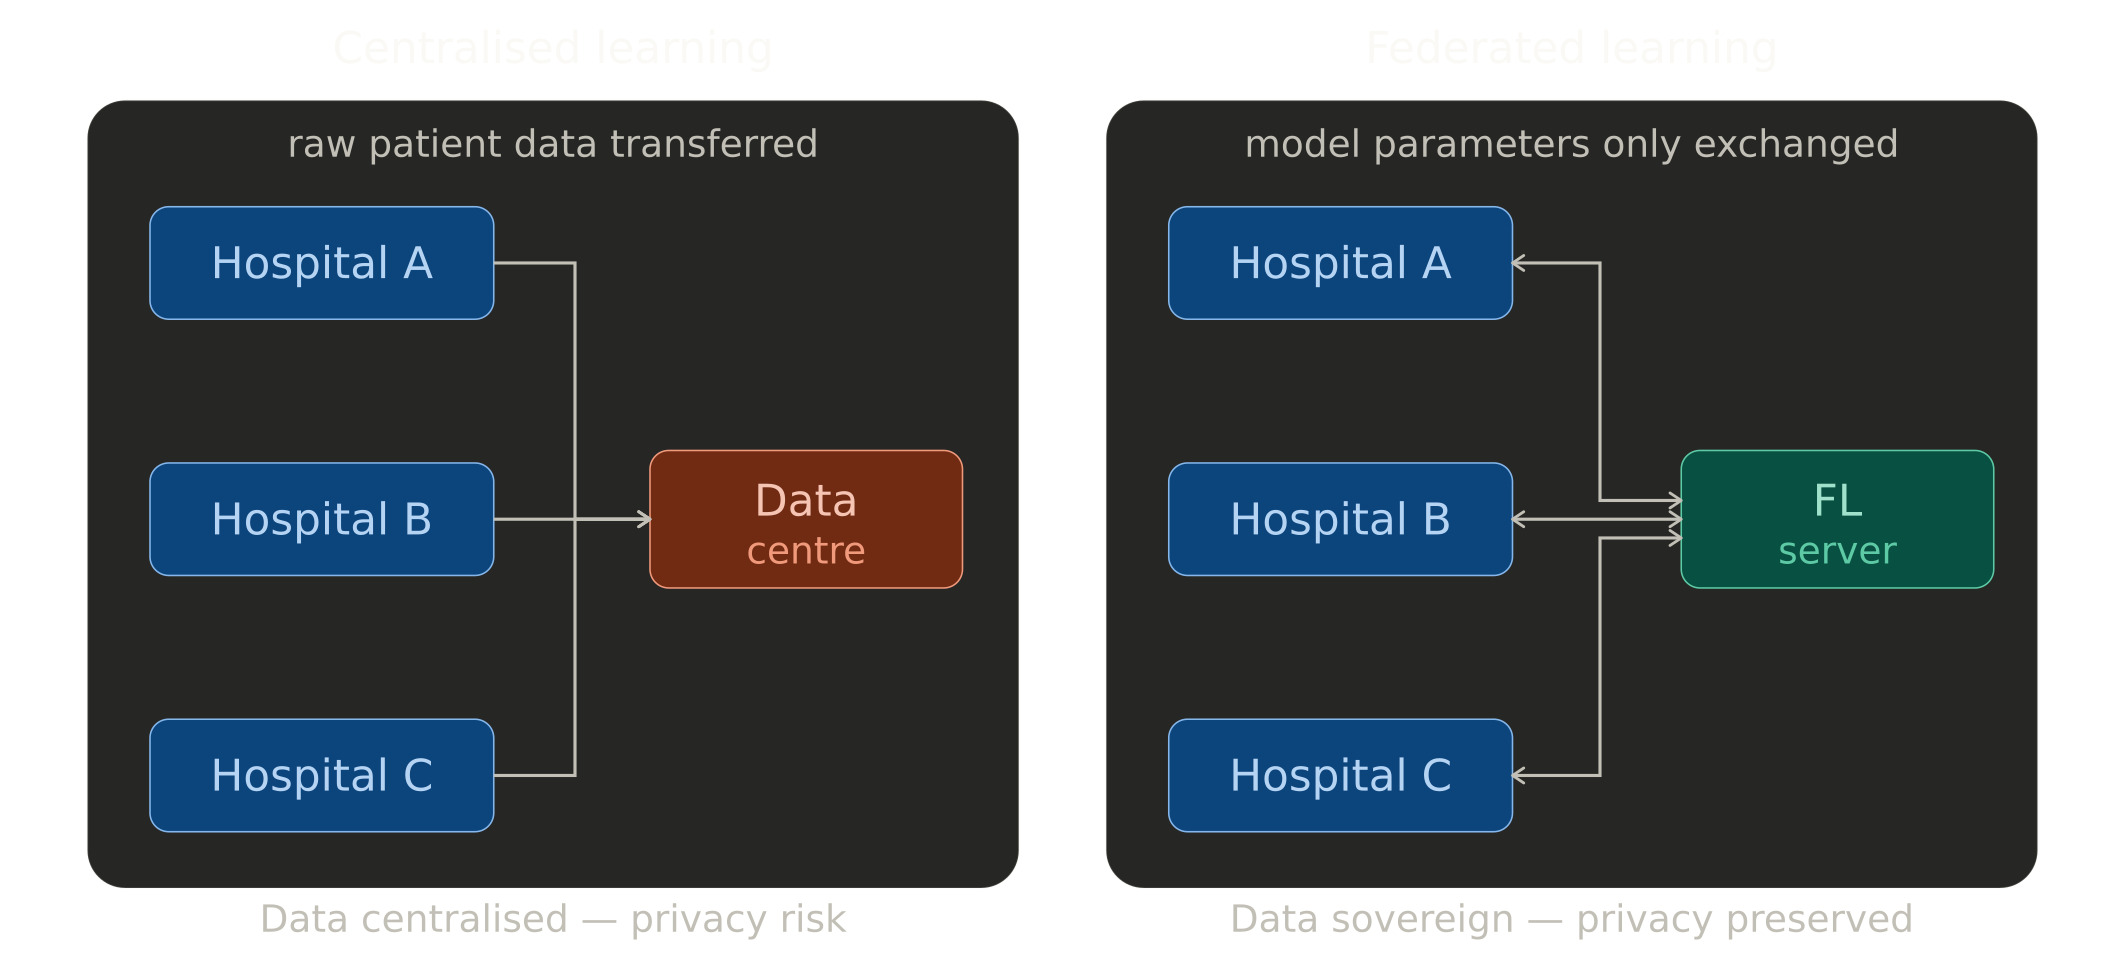
\includegraphics[width=\textwidth]{figures/fig2_1_centralised_vs_federated.jpg}
    \caption{Centralised versus federated learning in a multi-hospital
      breast MRI scenario. Left: raw patient data must be transferred
      to a single data centre, raising GDPR and data-sovereignty
      concerns \cite{gdpr2016regulation,hipaa1996health}. Right: only
      model parameters are exchanged with the coordination server;
      raw data remain at each institution \cite{mcmahan2017communication}.}
    \label{fig:centralised-vs-fl}
\end{figure}


\subsection{Distributed Learning Paradigms}
\label{sec:distributed-paradigms}

The limitations of centralised learning have motivated a spectrum of
distributed training approaches that differ in where data reside, how
computation is partitioned, and the degree of trust placed in the
coordinating infrastructure.
Understanding where federated learning sits within this spectrum
clarifies both its distinctive properties and the assumptions it makes.

\paragraph{Classical data-parallel distributed training.}
The most straightforward departure from single-machine training is
data-parallel processing in a parameter-server architecture
\cite{dean2012large}.
A central server maintains the canonical copy of model parameters;
a pool of worker machines each receive a disjoint shard of a centrally
stored dataset, compute gradients over that shard, and return the
gradients to the server for synchronous or asynchronous aggregation.
This architecture scales computation across many machines and has
become standard practice in industry for training large-scale models.
Crucially, however, the data themselves remain co-located in a shared
data centre under the exclusive control of a single operator.
Data-parallel distributed training therefore does not address the
privacy, sovereignty, or data-transfer cost concerns identified in the
previous section; it is an engineering technique for accelerating
computation over a centralised dataset, not a solution to the
multi-institutional data-governance problem.

\paragraph{Federated learning as a privacy-aware cross-silo paradigm.}
Federated learning introduces a qualitatively different constraint:
the training data are not co-located and, by design or by legal
requirement, cannot be moved to a central facility.
Each data silo -- referred to in the FL literature as a
\emph{client} -- retains its data locally and participates in the
training process by computing model updates on its own private dataset
and transmitting only those updates, never the raw data, to a
coordinating server \cite{mcmahan2017communication}.
The server aggregates parameter updates from participating clients and
broadcasts an improved global model for the next training round.
Raw patient records never traverse the network, and the communication
channel carries only floating-point model weights whose privacy
properties can be further reinforced with cryptographic or
noise-injection techniques (discussed in
Section~\ref{sec:privacy-security}).

FL is commonly classified along two orthogonal axes that determine the
applicable algorithms and privacy assumptions.
The first axis distinguishes \emph{horizontal} from \emph{vertical}
federation.
In \emph{horizontal} FL, all clients share the same feature space -- all
institutions acquire the same imaging modality and predict the same
outcome -- but hold non-overlapping patient populations.
This is the setting relevant to the present thesis: each of the three
simulated hospital clients holds a distinct cohort of breast MRI
patients with the same four molecular subtype labels.
In \emph{vertical} FL, clients hold overlapping patient identifiers
but complementary feature spaces -- for example, one institution holds
MRI images and another holds genomic profiles for the same patients.
Vertical federation requires patient-identifier alignment across sites,
which introduces additional privacy challenges and is a more complex
engineering problem \cite{yang2019federated,kairouz2021advances}.

The second axis distinguishes \emph{cross-device} from
\emph{cross-silo} federation.
Cross-device FL involves a very large number of lightweight,
intermittently available clients -- potentially millions of smartphones
or Internet-of-Things sensors -- communicating over unreliable
low-bandwidth links with highly heterogeneous hardware capabilities.
Cross-silo FL, by contrast, involves a small to moderate number of
institutional clients -- a consortium of hospitals or research
centres -- that are persistently available, possess substantial compute
resources, and are typically bound by formal data-sharing agreements
even if raw data transfer is prohibited.
The breast MRI classification scenario studied in this work corresponds
to \emph{cross-silo horizontal} FL: three simulated hospital clients,
each holding a non-IID partition of the 737-patient DCE-MRI dataset,
trained using the Flower framework with PyTorch as the local compute
backend.
Table~\ref{tab:fl-taxonomy} summarises the key distinctions between
the main FL paradigms.

\begin{table}[htbp]
  \centering
  \caption{Taxonomy of federated learning paradigms along two
    classification axes. This thesis operates in the cross-silo,
    horizontal quadrant.}
  \label{tab:fl-taxonomy}
  \renewcommand{\arraystretch}{1.3}
  \begin{tabular}{lll}
    \hline
    \textbf{Axis} & \textbf{Category} & \textbf{Characteristics} \\
    \hline
    \multirow{2}{*}{Data partition}
      & Horizontal FL & Same features, different patients \\
      & Vertical FL   & Same patients, complementary features \\
    \hline
    \multirow{2}{*}{Client scale}
      & Cross-device FL & Millions of clients; intermittent, heterogeneous \\
      & Cross-silo FL   & Tens of clients; persistent, institutional \\
    \hline
  \end{tabular}
\end{table}

\begin{figure}[htbp]
    \centering
    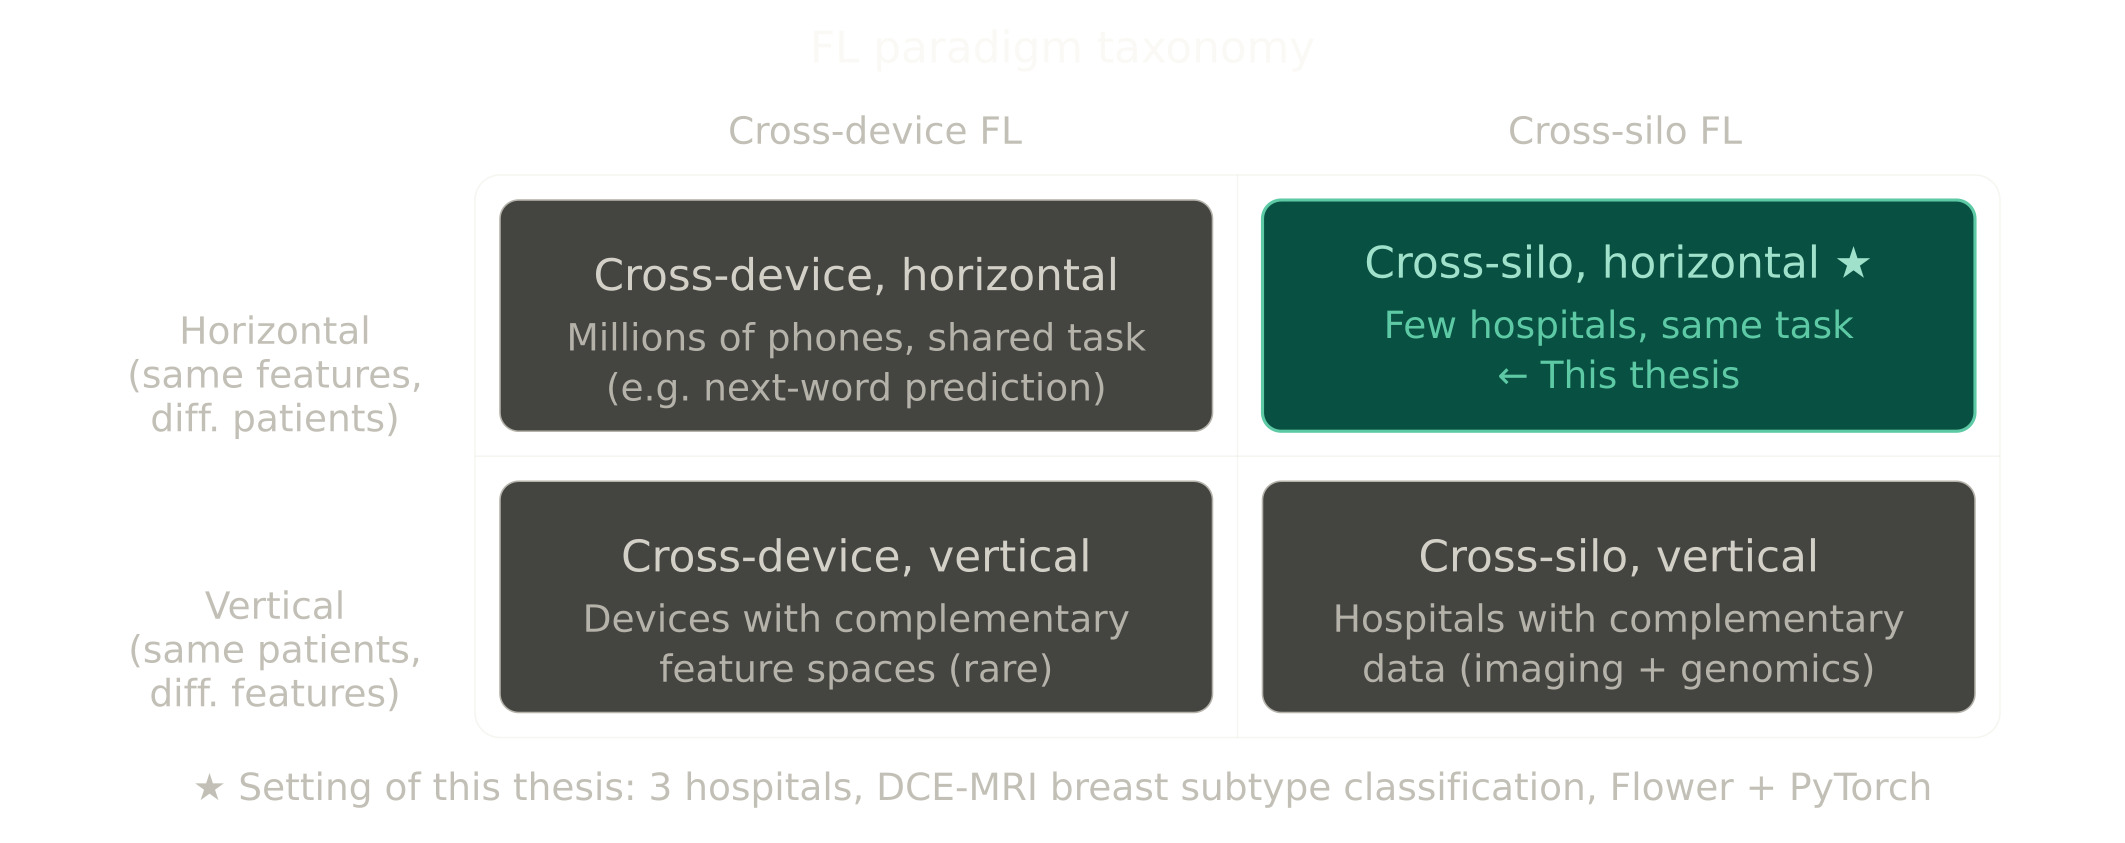
\includegraphics[width=0.8\textwidth]{figures/fig2_2_fl_taxonomy.jpg}
    \caption{Taxonomy of federated learning paradigms. The highlighted
      quadrant -- cross-silo, horizontal FL -- corresponds to the
      setting adopted in this thesis \cite{yang2019federated,kairouz2021advances}.}
    \label{fig:fl-taxonomy}
\end{figure}


\subsection{Definition and Origins of Federated Learning}
\label{sec:fl-definition}

Federated learning was formally introduced by McMahan \emph{et al.}\
in 2017 in the context of training a next-word-prediction language
model on data distributed across millions of mobile devices
\cite{mcmahan2017communication}.
The authors identified a class of learning problems characterised by
three properties: the training data are generated and stored on devices
that are not under the operator's direct control; those data contain
sensitive user information that makes centralised aggregation
undesirable; and the dataset is massively distributed, with each
device holding a relatively small and non-identically distributed
portion of the total information.
The proposed solution -- \emph{Federated Averaging} (FedAvg) -- has since
become the canonical baseline algorithm for the field and is described
in detail in Section~\ref{sec:fedavg}.

Formally, the federated learning optimisation problem is stated as
follows.
Let $K$ denote the number of participating clients, let
$\mathcal{D}_k$ denote the private local dataset of client $k$,
with $n_k = |\mathcal{D}_k|$ the number of local samples and
$n = \sum_{k=1}^{K} n_k$ the total sample count across all clients.
The goal is to find model parameters $\mathbf{w}^{\ast}$ that minimise
the globally weighted empirical risk:

\begin{equation}
  \mathbf{w}^{\ast}
  \;=\;
  \arg\min_{\mathbf{w} \in \mathbb{R}^d}
  \sum_{k=1}^{K} \frac{n_k}{n}\, F_k(\mathbf{w}),
  \label{eq:fl-objective}
\end{equation}

where the local objective $F_k$ of client $k$ is the empirical risk
over its private data:

\begin{equation}
  F_k(\mathbf{w})
  \;=\;
  \frac{1}{n_k}
  \sum_{(\mathbf{x},\, y)\,\in\,\mathcal{D}_k}
  \ell\bigl(f(\mathbf{x};\mathbf{w}),\; y\bigr),
  \label{eq:local-risk}
\end{equation}

with $f(\cdot\,;\mathbf{w})$ the model function parameterised by
$\mathbf{w}$, and $\ell$ the per-sample loss function (e.g.\
cross-entropy for multi-class classification).
The key observation is that the objective in
\eqref{eq:fl-objective} is \emph{mathematically equivalent} to
standard empirical risk minimisation over the pooled dataset
$\bigcup_k \mathcal{D}_k$, yet it can be minimised
\emph{without ever pooling the data} \cite{kairouz2021advances}.

Training proceeds in discrete \emph{communication rounds}.
At round $t$, the server selects a subset of clients
$\mathcal{S}^{(t)} \subseteq \{1,\ldots,K\}$ and broadcasts the
current global parameters $\mathbf{w}^{(t)}$.
Each selected client $k$ initialises its local model with
$\mathbf{w}^{(t)}$ and performs $E$ steps of mini-batch stochastic
gradient descent on $\mathcal{D}_k$, obtaining a locally updated
parameter vector $\mathbf{w}_k^{(t+1)}$.
The server then aggregates the client updates into a new global
model using a weighted average:

\begin{equation}
  \mathbf{w}^{(t+1)}
  \;=\;
  \sum_{k\,\in\,\mathcal{S}^{(t)}}
  \frac{n_k}{\displaystyle\sum_{j\,\in\,\mathcal{S}^{(t)}} n_j}\;
  \mathbf{w}_k^{(t+1)}.
  \label{eq:fedavg-aggregation}
\end{equation}

Equation~\eqref{eq:fedavg-aggregation} is the aggregation step of
FedAvg; the local training step and its interaction with data
heterogeneity are analysed in detail in Section~\ref{sec:aggregation}.

The transition from the original mobile cross-device setting to
cross-silo healthcare applications was both rapid and well-motivated.
Pioneering empirical work by Sheller \emph{et al.}\ demonstrated
that a FL model trained across multiple institutions, without any
data sharing, could achieve performance competitive with a centrally
trained baseline on a brain tumour segmentation task -- a result
attributable in part to the regularising effect of training on
heterogeneous clinical distributions \cite{sheller2020federated}.
Subsequent comprehensive surveys have catalogued FL applications
spanning radiology, pathology, genomics, and electronic health records
\cite{rieke2020future,nguyen2022federated,kaissis2020secure},
establishing federated learning as the dominant collaborative learning
paradigm endorsed by the medical AI research community when privacy
constraints prohibit raw data sharing.

\begin{figure}[htbp]
    \centering
    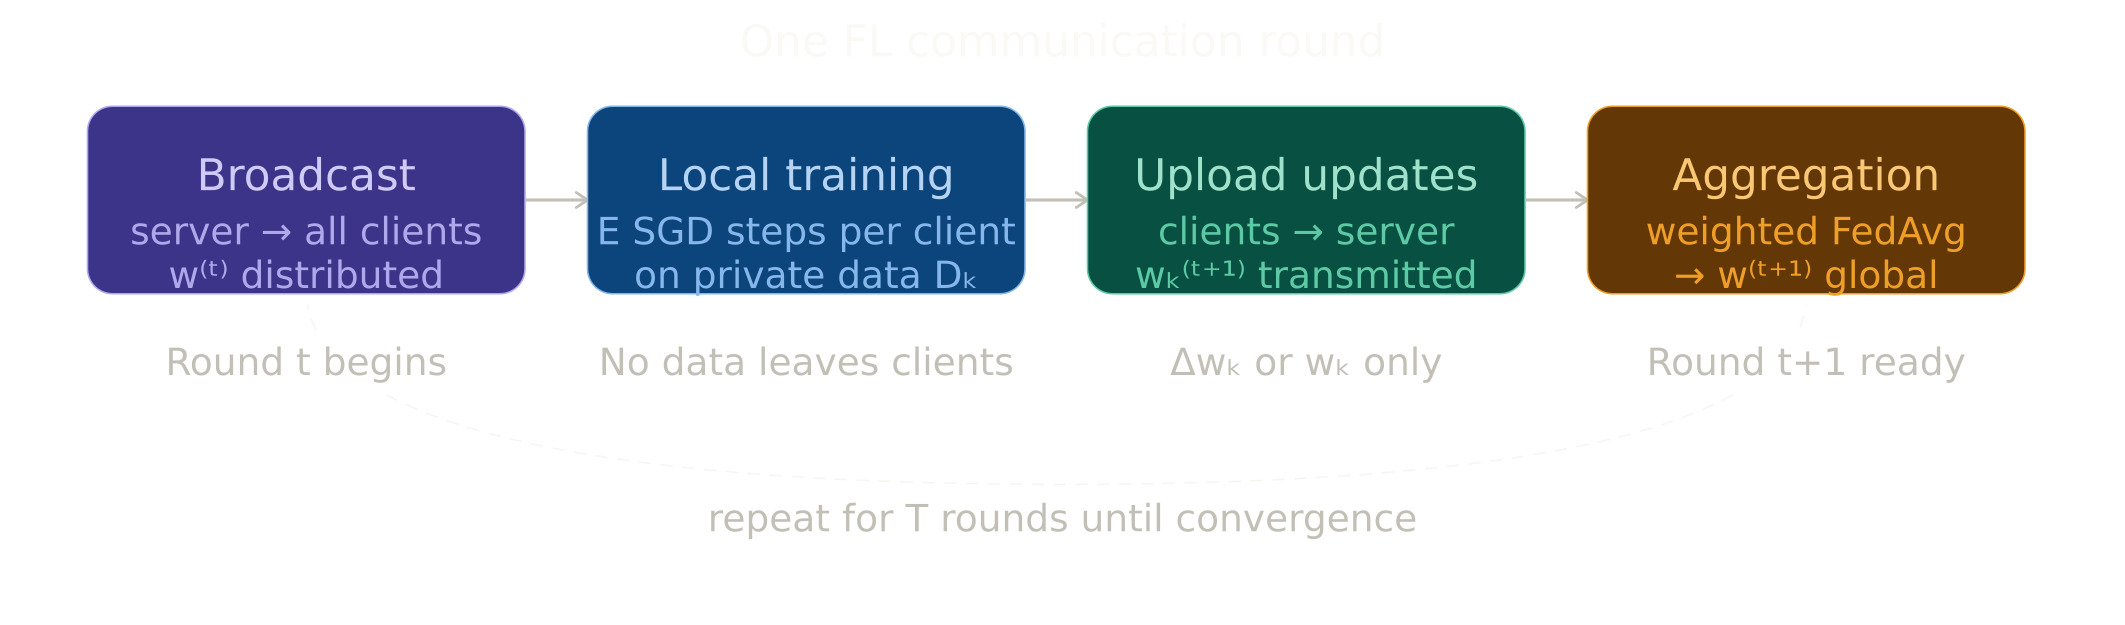
\includegraphics[width=\textwidth]{figures/fig2_3_one_fl_round.jpg}
    \caption{The four phases of one federated learning communication
      round (equation~\eqref{eq:fedavg-aggregation}). The server
      broadcasts $\mathbf{w}^{(t)}$, each client performs $E$ local
      SGD steps on $\mathcal{D}_k$, the resulting
      $\mathbf{w}_k^{(t+1)}$ are uploaded, and the server computes
      the weighted aggregate $\mathbf{w}^{(t+1)}$
      \cite{mcmahan2017communication,kairouz2021advances}.}
    \label{fig:fl-round}
\end{figure}


% ============================================================
\section{Federated Learning Architecture}
\label{sec:fl-architecture}
% ============================================================

The practical realisation of the federated optimisation objective
defined in Section~\ref{sec:fl-definition} requires a concrete system
architecture that coordinates communication between geographically
distributed participants, manages model state across training rounds,
and enforces the data-locality constraint that distinguishes federated
from centralised learning.
This section describes the canonical two-tier client--server
architecture that underlies most deployed and experimental FL systems,
including the Flower-based setup employed in this thesis.

\subsection{Client-Server Paradigm}
\label{sec:client-server}

The canonical FL architecture is organised as a two-tier hierarchy
consisting of a central coordination server and a set of $K$ clients,
each in possession of a private local dataset $\mathcal{D}_k$ that
remains on-site throughout the entire training process
\cite{mcmahan2017communication}.
The server is the orchestrating entity: it maintains the authoritative
copy of the global model, schedules training rounds, selects
participating clients, aggregates locally computed updates, and
broadcasts the updated global model.
Clients are the computational entities: each executes local
optimisation on its own data and returns parameter updates to the
server without exposing raw records.

This division of responsibility reflects both the privacy requirement
and the typical infrastructure of cross-silo healthcare deployments.
The server may be hosted by a neutral third party -- a research
consortium, a cloud provider operating under a data-processing
agreement, or one of the participating hospitals designated as
coordinator -- provided that the server never receives raw patient data.
Clients in a cross-silo setting are typically individual hospital sites
or research centres, each equipped with sufficient GPU compute to
execute local training on their imaging datasets
\cite{rieke2020future,kairouz2021advances}.

An important architectural distinction concerns the degree of client
selection per round.
In large-scale cross-device FL, only a small fraction of available
clients participate in each round due to device availability and
bandwidth constraints.
In cross-silo deployments of the kind considered in this thesis, where
the total number of clients is small (three simulated hospital nodes),
all clients participate in every round, simplifying convergence
analysis and eliminating the client-dropout variability that
complicates cross-device FL \cite{kairouz2021advances}.

\subsection{Local Training at Client Institutions}
\label{sec:local-training}

At the commencement of each communication round $t$, every selected
client $k \in \mathcal{S}^{(t)}$ receives the current global parameter
vector $\mathbf{w}^{(t)}$ from the server and initialises its local
model with this shared starting point.
The client then performs a fixed number $E$ of local optimisation
steps using mini-batch stochastic gradient descent (SGD) over its
private dataset $\mathcal{D}_k$, minimising the local empirical risk
$F_k(\mathbf{w})$ defined in equation~\eqref{eq:local-risk}.

The choice of $E$ governs the trade-off between communication
efficiency and optimisation quality.
A single local step ($E = 1$) reduces to synchronous distributed SGD
and requires a communication round after every gradient computation,
incurring high bandwidth costs.
Multiple local steps ($E > 1$) amortise the communication overhead
across more computation but introduce \emph{client drift}: because
each client optimises its local objective rather than the global one,
the local model moves away from the global optimum at a rate that
depends on the statistical heterogeneity of the local data distribution
\cite{kairouz2021advances}.
In the non-IID setting characteristic of multi-hospital deployments --
where patient demographics, scanner protocols, and subtype prevalence
differ across sites -- client drift is a primary source of convergence
degradation and motivates the regularisation techniques discussed in
Section~\ref{sec:aggregation}.

In the breast MRI molecular subtype classification scenario of this
thesis, each client applies the same ResNet-based backbone architecture
initialised from the global weights, performing local updates using a
cosine learning rate schedule with MixUp augmentation to mitigate the
class imbalance arising from the non-IID partition of the 737-patient
dataset across three hospital nodes.
Progressive unfreezing of backbone layers during local training is
employed to preserve low-level feature representations learned from the
global model while adapting higher-level features to site-specific data
characteristics.

\subsection{Global Model Aggregation on the Server}
\label{sec:global-aggregation}

Upon completion of local training, each participating client $k$
transmits its updated local parameter vector $\mathbf{w}_k^{(t+1)}$
to the central server.
The server's aggregation function combines these client updates into a
new global model that, under the weighted averaging scheme of FedAvg,
corresponds to the sample-size-weighted mean of local parameters as
given in equation~\eqref{eq:fedavg-aggregation}.
The resulting global model $\mathbf{w}^{(t+1)}$ integrates knowledge
from all participating clients without requiring any client to share
its underlying data.

The correctness of weighted averaging as an aggregation operator rests
on the assumption that local models are trained from the same
initialisation and that the global objective is the weighted sum of
local objectives with weights proportional to dataset size
\cite{mcmahan2017communication}.
Under these conditions, averaging in parameter space approximates a
single gradient step on the global objective.
When the assumption of identical data distributions across clients is
violated -- the non-IID case -- this approximation degrades, and the
aggregated model may converge to a point that is suboptimal for all
clients simultaneously.
Alternative aggregation strategies that address this degradation are
surveyed in Section~\ref{sec:aggregation}.

A practical consideration in cross-silo medical imaging deployments is
the size of the parameter vectors being transmitted.
A ResNet-50 backbone comprises approximately 25 million floating-point
parameters; transmitting full parameter vectors from three hospital
clients per round is feasible within the bandwidth constraints of
institutional networks, in contrast to the gradient-compression
requirements of cross-device deployments involving thousands of
participants \cite{kairouz2021advances,rieke2020future}.

\subsection{Communication Rounds and Convergence}
\label{sec:comm-rounds}

Training in federated learning is structured as a sequence of discrete
communication rounds rather than the continuous gradient flow of
centralised training.
Each round consists of four steps: the server broadcasts the current
global model to selected clients; clients perform local optimisation;
clients transmit updated parameters to the server; and the server
aggregates the updates and prepares the next global model.
This round structure introduces a fundamental coupling between the
number of communication rounds $T$, the number of local steps $E$ per
round, and the total computational budget available to each client.

Convergence analysis for FedAvg under non-IID data distributions
demonstrates that the algorithm converges at a rate that degrades as
the degree of data heterogeneity -- measured by the gradient divergence
$\|\nabla F_k(\mathbf{w}) - \nabla F(\mathbf{w})\|$ across clients --
increases \cite{kairouz2021advances}.
Intuitively, when local data distributions differ substantially, local
gradient directions point towards different local optima, and their
average after multiple local steps is a poor approximation to the
global gradient.
The practical consequence is that non-IID FL systems may require
significantly more communication rounds to achieve a given target
accuracy than an equivalent centralised system trained on the pooled
dataset.

In healthcare FL deployments, the number of communication rounds is
also constrained by institutional factors beyond pure optimisation
considerations: each round involves synchronisation across hospital
sites that may operate on different schedules, under different
computational loads, and subject to network availability constraints
that do not arise in a single data centre.
For the three-hospital simulation in this thesis, all clients are
available synchronously, so round scheduling reduces to a hyperparameter
choice; the interaction between round count, local epochs, and
convergence on the non-IID breast MRI partition is reported in
Chapter~3.


% ============================================================
%  STUB SECTIONS 2.4 -- 2.10
%  Labels only -- prose to be filled in progressively.
%  Do NOT remove these stubs until the section is fully written;
%  they resolve all forward \ref{} calls from sections above.
% ============================================================

\section{Aggregation Strategies}
\label{sec:aggregation}
% TODO: Write section 2.4 (FedAvg variants, FedProx, FedNova, SCAFFOLD, personalised FL)

\subsection{Federated Averaging}
\label{sec:fedavg}
% TODO: Write 2.4.1 -- detailed FedAvg walkthrough (referenced from sec:fl-definition)

\section{Communication Protocols and Optimisation}
\label{sec:communication}
% TODO: Write section 2.5 (gradient compression, quantisation, asynchronous FL)

\section{Privacy and Security in Federated Learning}
\label{sec:privacy-security}
% TODO: Write section 2.6 (threat models, DP, secure aggregation, HE)

\section{Convergence and Stability Challenges}
\label{sec:convergence}
% TODO: Write section 2.7 (non-IID impact, system heterogeneity, stabilisation)

\section{Federated Learning Frameworks}
\label{sec:frameworks}
% TODO: Write section 2.8 (Flower, FedML, Substra, PySyft, comparison)

\section{Related Work}
\label{sec:related-work}
% TODO: Write section 2.9 (FL in EEG, medical imaging, oncology; positioning)

\section{Conclusion}
\label{sec:ch2-conclusion}
% TODO: Write section 2.10
